\documentclass{report}
\usepackage[margin=1in]{geometry}
\usepackage{setspace}
\usepackage{times}
\usepackage{pdfpages}
\title{
	\textsc{ \small
		Washington State University \\
		School of Electrical Engineering and Computer Science \\
		EE 352, Electrical Engineering Laboratory
	} \\
	{\textsc{\small Lab \#2}} \\
	State Variable Modeling and Mutual Inductance
}

\author{
	Name: Kevin Evans \\
	Partner: Jacob Hnatiak
}
\date{Due Date: February 4, 2020}


% start sections at 1 with subsections to 1.1, 1.2...
\renewcommand{\thesection}{\arabic{section}}

%alias for vpp/rms
\newcommand{\pp}{_{pp}}
\newcommand{\rms}{_{rms}}
\newcommand{\Vpp}{\V\pp}
\newcommand{\Vrms}{\V\rms}

\usepackage{pgfplots}
\usepackage{filecontents}

\usepackage{clipboard}
\usepackage{siunitx}
\usepackage{threeparttable}
\usepackage{booktabs}
\usepackage{multirow}
\usepackage{graphicx}
\usepackage{float}
\usepackage{amssymb,amsmath}
\usepackage{physics,cancel}

\usepackage{steinmetz} % \phase{}
\usepackage{mathtools} % for '\mathclap' macro
\usepackage{caption,subcaption} %multiline captions; subfigures

\sisetup{inter-unit-product=\cdot}

\usepgfplotslibrary{units}

\begin{document}
\maketitle

\section*{Lab Overview}
% what was the lab about and the outcome?
In this lab, two experiments were done: one was to determine the mutual inductance of a transformer circuit, and the other was to use state variables to model a RLC circuit. The mutual inductance was found using a triangular wave input as well as an input phasor, and averaged to find the coupling coefficient. The RLC circuit was modeled using OrCAD initially and the model was confirmed experimentally. Next, a MATLAB model was created using state variables and it was found to be within 5\% of the actual circuit response.

\section{Mutually coupled transformer circuit}

\subsection{Purpose}
% purpose of the experiment and its specs and/or design requirements
The purpose of this experiment was to experimentally determine the mutual inductance $M$ between two inductors in a transformer circuit. This was done using two methods: by measuring the sinusoidal response and the step response.

\subsection{Theoretical background}
% background and its theory of operation, circuit diagrams, the main equations, results from the prelab

Inductors can share a magnetic flux, when two are placed relatively nearby. This is often seen in transformers, which can step down or up a potential, using this coupling. In this experiment, the circuit shown in Figure \ref{fig:mutualinductors} was assembled to experimentally determine the mutual inductance of two inductors, $L_1$ and $L_2$.

\begin{figure}[h]
	\centering
	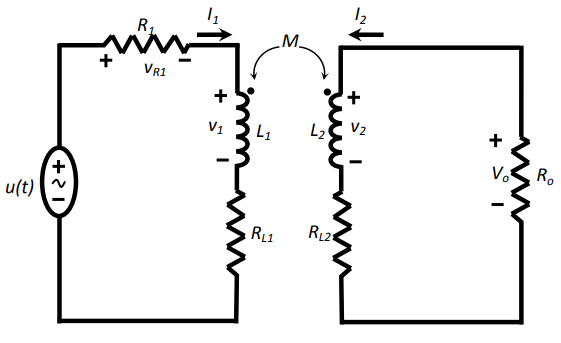
\includegraphics[width=0.6\linewidth]{mutualinductors}
	\caption{The circuit diagram used in this experiment.}
	\label{fig:mutualinductors}
\end{figure}

\subsubsection{Triangular wave: constant change in current}
From here, we can generate a triangular wave from $u(t)$, with a constant ramping in voltage. If we set $R_o \to \infty$, it acts as an open circuit and no current flows in the second loop, $I_2$.
In the time domain, for this coupled inductor pair, the voltages across each are given as
\begin{subequations}
	\label{eq:1voltages}
	\begin{align}
		v_1(t) & = L_1 \dv{i_1}{t} + \cancel{M \dv{i_2}{t}} \\
		v_2(t) & = M \dv{i_1}{t} + \cancel{L_2 \dv{i_2}{t}} \label{eq:1voltage}
	\end{align}
\end{subequations}

Thus, if we measure only the current $I_2$ and the potential across $v_o$, we can determine the mutual inductance $M$. We additionally will make further assumptions: the resistance of coil 1 $R_{L1}$ will be much less than $R_1$, and will be negligible in the calculations. Additionally, we will assume that $V_{R1}$ will be equal to $u(t)$---as the voltage drop across $L_1$ will be minimal (this will be demonstrated in the sinusoidal response).

As a triangular wave is being used, we can assume that the current in the left loop, $I_1$, will follow 
\begin{equation}
	\dv{i_1}{t} = \frac{1}{R_1} \dv{V_{R1}}{t} \approx \frac{1}{R_1} \frac{\Delta V_{R1}}{\Delta t} \label{eq:1didt}
\end{equation}
where $\Delta I_1$ is the difference between the peak current values. This is expected to be constant as the voltage across $L_1$ was neglected from the earlier assumptions.
For a \SI{10}{\Vpp} triangular pulse at \SI{400}{\Hz} across resistor $R_1$, the current differential \eqref{eq:1didt} evaluates to \begin{equation}
	\dv{i_1}{t} = 2 \cross (\SI{400}{\Hz}) \cross \frac{\SI{10}{\Vpp}}{\SI{10}{\kohm}} = \pm \SI{0.8}{\A\per\s}
\end{equation}
Equating this with \eqref{eq:1voltage}, if the voltage across the right loop $v_2$ is measured and the difference between the peak-to-peak voltage is calculated as $\Delta V_2$, we can determine the mutual inductance as 
\begin{equation}
	M = \frac{\Delta V_2}{\dv{i_1}{t}} \label{eq:mtriangle} %\frac{\Delta V_2 R_1}{800 \Delta V_1}
\end{equation}

\subsubsection{Sinusoidal response}
Next, to determine the sinusoidal response, we can characterize the inductor voltage drop using impedances. Once again, the $I_2$ becomes zero as the output resistance is modeled as infinite,
\begin{subequations}
	\begin{align}
		V_1 & = j \omega L_1 I_1 + \cancel{j \omega M I_2} \\
		V_2 & = j \omega M I_1 + \cancel{j \omega L_2 I_2} \label{eq:1v2}
	\end{align}
\end{subequations}
Next, we calculate the impedance of the left-hand loop using ideal values of \begin{align*}
	L_1 = L_2 & = \SI{200}{\milli\henry} \\
	R_\mathrm{L1} = R_\mathrm{L2} & = \SI{50}{\ohm} \\
	R_1 & = \SI{10}{\kohm} \\
	R_o & = \infty \\
	u(t) & = \SI{10}{\Vpp} \phase{0^\circ} && \omega=\SI{400}{\Hz} \\
	V_1 & = V_m \phase{\theta} && \omega = \SI{400}{\Hz}
\end{align*}
Then, the impedance of the left-hand loop is \begin{subequations}
	\begin{align}
		Z_\mathrm{LHS} & = Z_\mathrm{R1} + Z_\mathrm{L} \\
			& = R_1 + j\omega L_1 + R_\mathrm{L1}
	\end{align}
\end{subequations}
However, relative to $R_1$, the impedance of the inductor $Z_L$ is minuscule and can be neglected. The current will primarily be dictated by the magnitude of $R_1$, as $Z_\mathrm{LHS} \approx R_1$ for the ideal values. Then, the current $I_1$ can be calculated as
\begin{equation}
	I_1 = \frac{u(t)}{Z_\mathrm{LHS}} = \frac{V_1}{R_1} \label{eq:1current2}
\end{equation}
Combining \eqref{eq:1v2} and \eqref{eq:1current2}, the inductor coupling can be determined as
\begin{equation}
	M = \frac{\abs{V_2}}{\omega \abs{I_1}} = \frac{V_2}{\omega V_1 / R_1} \label{eq:msine}
\end{equation}

\pagebreak
\subsection{Procedure}
The follow steps were carried out, as instructed by the lab assignment.
\begin{enumerate}
	\item Two inductors were chosen (from the lab cabinets). Their inductance and resistances were recorded using the RLC meter.
	\item The transformer circuit was constructed per Figure \ref{fig:mutualinductors}.
	\item A \SI{4}{\Vpp} triangular pulse \SI{400}{\Hz} was generated using the function generator and attached to points $u(t)$ on the circuit diagram.
	\item A tee was used to split the input signal into CH1 of the oscilloscope. CH2 was attached across inductor $L_1$ and CH3 was attached to the output voltage, $V_2$. All were set to 1X.
	\item To reduce noise, CH3 was set to average every 4 samples. On the oscilloscope, \texttt{Acquire} $\rightarrow$ \texttt{Average} $\rightarrow$ CH3: 4 samples.
	\item Resistor $R_1$ acted as a shunt to estimate the loop current. This was done by using the \texttt{Math} feature on the oscilloscope and setting it to subtract CH1 (input voltage) and CH2 (the inductor voltage), then the resistor current was estimated using this difference. \label{step:shunt}
	\item This was demonstrated to the TA and checked off.
	\item Next, a \SI{10}{\Vpp} sinusoidal wave was generated and the current was estimated using the same method as Step \ref{step:shunt}. The oscilloscope outputs were recorded and saved.
	\item The mutual inductance was estimated using \eqref{eq:mtriangle} and \eqref{eq:msine}.
\end{enumerate}

\subsection{Results and analysis}
% state all measured values, graphs, tables, and figs.
% state any deviation from theoretical expected values
% use tables and graphs
% * must justify error in results otherwise the experiment failed

\subsubsection{Experimental component values}
The measured component values are shown in Table \ref{table:lab1components}.

\begin{table}[h]
	\centering
	\caption{Experimental and nominal component values.}
	\begin{threeparttable}
		\begin{tabular}{cccc}
			\toprule
			Component & Nominal & Experimental & \% Error (Tolerance) \\
			\midrule
			$L_1$\tnote{1}  & -- & \SI{173}{\milli\henry} & -- \\
			$L_2$\tnote{1}    & -- & \SI{175}{\milli\henry} & -- \\
			$R_{L1}$ & -- & \SI{72.83}{\ohm} & -- \\
			$R_{L2}$ & -- & \SI{73.33}{\ohm} & -- \\
			$R_1$ & \SI{10}{\kohm} & \SI{9.738}{\kohm} & 2.6\% (5\%) \\
			\bottomrule
		\end{tabular}
		\begin{tablenotes}
			\footnotesize
			\item[1] $L_1$ and $L_2$ were labeled as \#13 and \#6 respectively.
		\end{tablenotes}
	\end{threeparttable}
		\label{table:lab1components}
\end{table}

\subsubsection{Triangular wave mutual inductance calculation}
The instantaneous change in current $I_1$ was found by measuring the peak-to-peak voltage across $R_1$ using the oscilloscope, shown in Figure \ref{fig:1scope} This was applied using \eqref{eq:1didt} and recorded. The peak-to-peak voltage across $L_2$ was measured, shown in Figure \ref{fig:1scope}, and recorded as $V_2$. This value was halved in \eqref{eq:1m}, as the magnitude is needed. Using \eqref{eq:mtriangle}, the instantaneous change in current and mutual inductance can be found as
\begin{subequations}
	\begin{align}
		\dv{I_1}{t} & = \frac{1}{R_1} \dv{V_{R1}}{t} = \frac{1}{\SI{9.738}{\kohm}} \frac{\SI{9.84}{\V}}{\SI{1.25}{\ms}} = \SI{0.808}{\A\per\s} \\
		M & = \frac{V_2}{\dv{I_1}{t}} = \frac{\SI{49.2}{\mV} / 2}{\SI{0.808}{\mA\per\s}} = \SI{30.45}{\milli\henry} \label{eq:1m}
	\end{align}
\end{subequations}

\begin{figure}[H]
	\begin{minipage}{0.5\linewidth}
		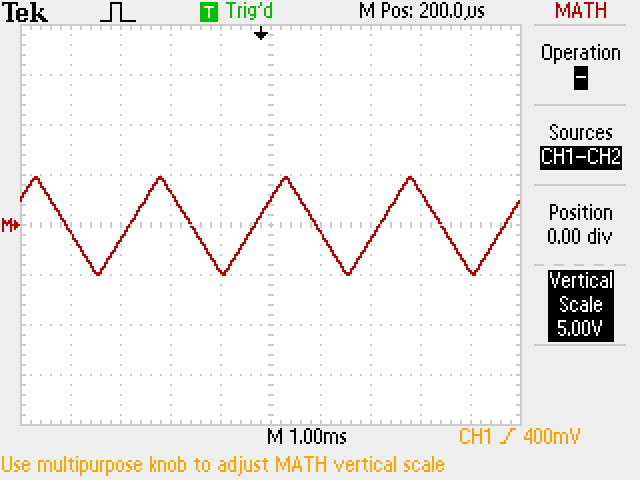
\includegraphics[width=\linewidth]{scope/ramp_vr}
	\end{minipage}
	\begin{minipage}{0.5\linewidth}
		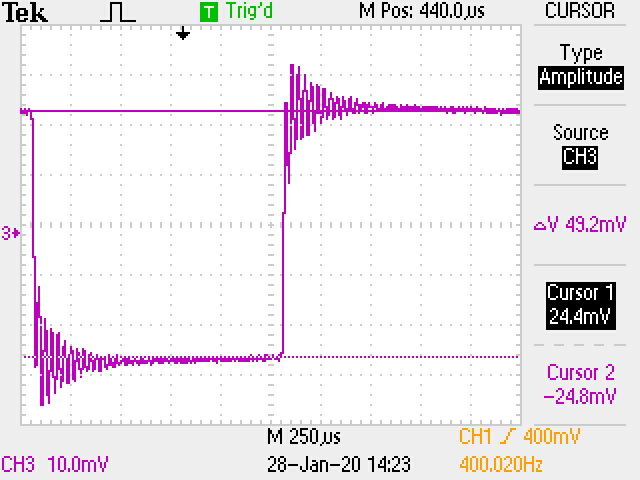
\includegraphics[width=\linewidth]{scope/ramp_v2}
	\end{minipage}
	\caption{The voltage across the shunt resistor $R_1$ (left) and inductor $L_2$ (right).}
	\label{fig:1scope}
\end{figure}

\subsubsection{Sinusoidal wave mutual inductance calculation}
In the latter half of the experiment, a sine wave was used and the mutual inductance was measured. Shown in Figure \ref{fig:1scopesine}, the voltage $V_2$ across inductor $L_2$ was measured,
\begin{align}
	V_2 & = \SI{65.6}{\mV} && \text{(peak-to-peak)} \notag \\
		& = \SI{32.8}{\mV} && \text{(zero-to-peak)}
	\intertext{The voltage $V_{R1}$ across the shunt was measured and the magnitude of the current $I_1$ was calculated as}
	I_1 & = \frac{V_{R1}}{R_1} = \frac{\SI{9.84}{\V}}{\SI{9.738}{\kohm}} = \SI{1.01}{\mA} && \text{(peak-to-peak) } \notag \\
	& = \SI{0.51}{\mA} && \text{(zero-to-peak)}
	\intertext{From these, the mutual inductance was calculated using \eqref{eq:msine},}
	M & = \frac{\SI{32.8}{\mV}}{\left(\SI{800 \pi}{\radian\per\sec} \right) \left(\SI{0.51}{\mA}\right)} \notag \\
		& = \SI{25.60}{\milli\henry}
\end{align}

\subsubsection{Average mutual inductance and coupling coefficient}
The average mutual inductance using the two methods was found as \begin{align}
	\bar{M} & = \frac{30.45 + 25.60}{2} \notag \\
		& = \SI{28.03}{\milli\henry}
\end{align}
Using the inductor values from Table \ref{table:lab1components}, the coupling coefficient can be estimated, \begin{align}
	k & = \frac{\bar{M}}{\sqrt{L_1 L_2}} =  \frac{28.03}{\sqrt{173 \times 175}} \qquad [\si{\milli\henry/\milli\henry}]\notag \\
		& = 0.161
\end{align}

\begin{figure}[H]
	\begin{minipage}{0.5\linewidth}
		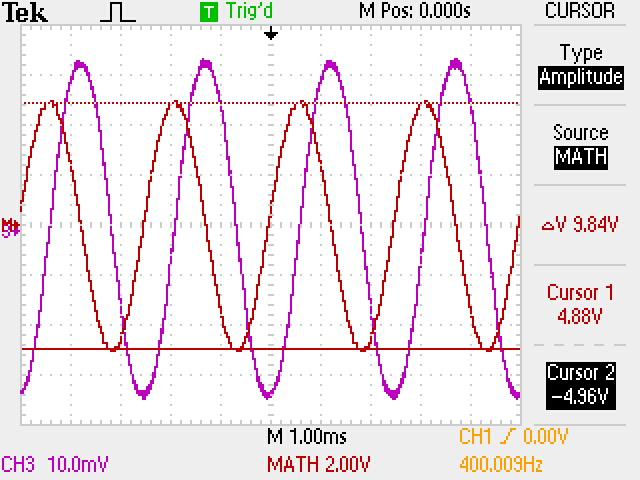
\includegraphics[width=\linewidth]{scope/sine_vr}
	\end{minipage}
	\begin{minipage}{0.5\linewidth}
		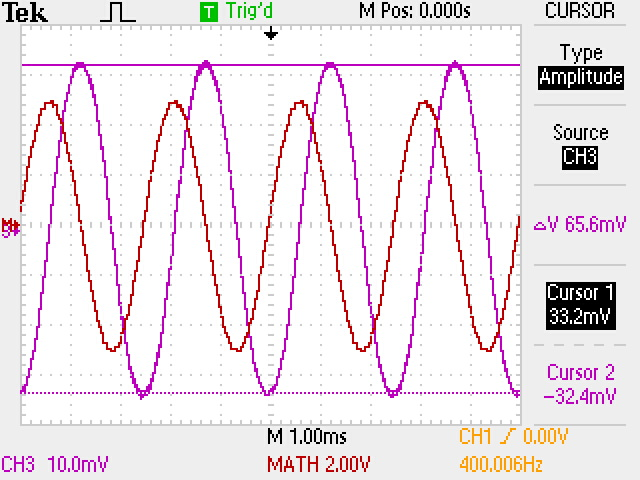
\includegraphics[width=\linewidth]{scope/sine_v2}
	\end{minipage}
	\caption{The voltage across the shunt resistor $R_1$ (left) and inductor $L_2$ (right).}
	\label{fig:1scopesine}
\end{figure}

\subsubsection{Inductor dot notation}
The dot notation of the circuit shown in Figure \ref{fig:rlccircuit} is backwards in inductor $L_2$, and the dot should be placed at the negative terminal of $V_2$. This is evident in Figure \ref{fig:1dot} as the voltages across each inductor are half a cycle out of phase. Once inductor $L_2$ was reversed, the voltages became nearly in-phase.

\begin{figure}[H]
	\centering
	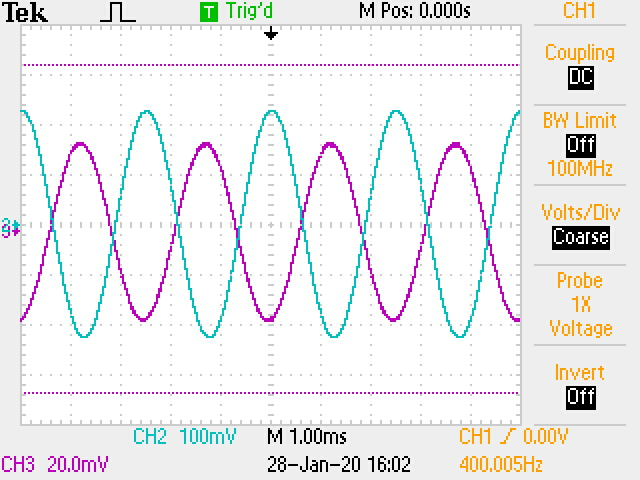
\includegraphics[width=0.5\linewidth]{scope/dot}
	\caption{The voltage across inductor $L_1$ (blue) and $L_2$ (fuchsia).}
	\label{fig:1dot}
\end{figure}

\subsection{Conclusion}
%  conclusion of the exp
This experiment found a mutual inductance using two methods: a triangular input response with constant current slope, and a sinusoidal phasor input and phasor response. There was a fairly large difference between the two and the average. Between the two calculated $M$ values and the mean $\bar{M}$, there was $8.7\%$ and $8.5\%$ error using the triangular and sinusoidal response respectively. The difference between these two experiments could be due to several factors, but we believe the error came from the poor alignment of the inductors. During the experiment, it was noticed that barely nudging each transformer, even if moved a millimeter, would have a substantial effect on the output voltage of inductor $L_2$.

%%%%%%%%%%%%%%%%%%%%%%%%%%%%%%%%%%%%%%%%%%%%%%%%%%%%%%%%%%%%%%%%%%%%%%%%%%%%%%%%%%%%%%%%%%%%%%%%%%%%%%

\pagebreak

\section{State variable modeling of RLC circuits}

\subsection{Purpose}
% purpose of the experiment and its specs and/or design requirements
The purpose of this experiment was to solve for voltages and currents in a linear circuit using state variable models. In the experiment, we modeled an RLC circuit containing parallel RLC components.
\subsection{Theoretical background}
% background and its theory of operation, circuit diagrams, the main equations, results from the prelab
Circuits containing linear components can be modeled using the state variables, where capacitor voltages and inductor currents are set as continuous state variables. The derivatives of these state variables can be used to determine how other variables evolve over time in the circuit. Here, we use a state variable model to inspect the voltage across a capacitor and the current through an inductor, and determine the response of the system as a whole.

We can model the circuit in Figure \ref{fig:rlccircuit} using state variables. In this instance, the state variables are $x_1(t) = v_c(t)$  and $x_2(t) = i_L(t)$. We can use KVL/KCL to determine the relation between $x_1$ and $x_2$ and their interaction in the circuit. From this, we can produce the matrices\footnote{The derivation for this is found in Appendix C of the lab handout.} to find solutions to the circuit, \begin{equation}
	\underbrace{ \left[ \begin{matrix}
		\dot{x}_1(t) \\
		\dot{x}_2(t)
	\end{matrix} \right] }_{\mathbf{\dot{X}}}
	=
	\underbrace{ \left[
		\begin{matrix}
			-\frac{1}{C(R_s + R_1)} & -\frac{1}{C} \\
			\frac{1}{L} & -\frac{R_2 + R_L}{L}
		\end{matrix}
	\right] }_{\mathbf{A}}
	\underbrace{ \left[
		\begin{matrix}
			x_1(t) \\
			x_2(t)
		\end{matrix}
		\right]
	}_{\mathbf{X}}
	+
	\underbrace{
		\Copy{copy:mtx}{
			\left[ \begin{matrix}
				\frac{1}{C(R_s + R_1)} \\
				0
				\end{matrix}
			\right]
		}
	}_\mathbf{B}
	\underbrace{
		\vphantom{ \Paste{copy:mtx} }
		\left(
			u(t) \times
			\mathbf{I}_2
		\right)
	}_{\mathclap{\mathbf{G}}}
	\label{eq:poop}
\end{equation}
Next, we can simulate the circuit in OrCAD PSPICE. The circuit was modeled in OrCAD using the nominal values in Figure \ref{fig:rlccircuit}. A step response with pulse width of \SI{5}{\ms} was used as it would allow the RLC circuit ample time to reach equilibrium. The simulation shows ringing occurring on both state variables before reaching equilibrium at $x_1 = \SI{255.9}{\mV}$ and $x_2 = \SI{82.6}{\mA}$. The full result of the simulation is shown in Figure \ref{fig:rlcsim} (Appendix).
\begin{figure}[h]
	\centering
	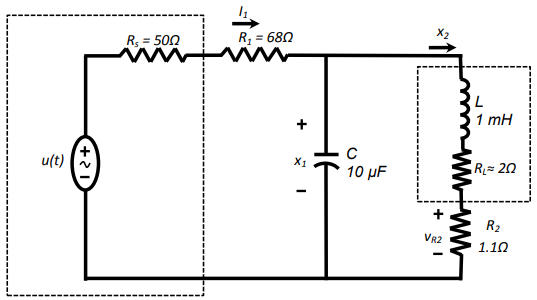
\includegraphics[width=0.6\linewidth]{rlccircuit}
	\caption{The RLC circuit used in this experiment.}
	\label{fig:rlccircuit}
\end{figure}

\subsection{Procedure}
The follow steps were carried out, as instructed by the lab assignment.
\begin{enumerate}
	\item The values for the components in Figure \ref{fig:rlccircuit} were recorded.
	\item A square wave of \SI{10}{\Vpp} and \SI{5}{\V} offset was generated. This was equivalent to an input of $10 u(t)$.
	\item The frequency was set to $\SI{20}{\Hz}$ as it gave the best results.
	\item The waveforms and points were captured and saved to a flash drive from the oscilloscope. In Excel, the trajectory was plotted.
\end{enumerate}

\subsection{Results and analysis}
% state all measured values, graphs, tables, and figs.
% state any deviation from theoretical expected values
% use tables and graphs
% * must justify error in results otherwise the experiment failed

\subsubsection{Experimental component values}
The measured component values are shown in Table \ref{table:lab2components}.

\begin{table}[h]
	\centering
	\caption{Experimental and nominal component values.}
	\label{table:lab2components}
	\begin{threeparttable}
		\begin{tabular}{cccc}
			\toprule
			Component & Nominal & Experimental & \% Error (Tolerance) \\
			\midrule
			$L$  & \SI{1}{\milli\henry} & \SI{1.146}{\milli\henry} & 4.1\%  \\
			$R_L$ & -- & \SI{2.23}{\ohm} & -- \\
			$R_1$ & \SI{68}{\ohm} & \SI{67.42}{\ohm} & 0.08\% (10\%) \\
			$R_2$ & \SI{1.1}{\ohm} & \SI{1.20}{\ohm} & 9.1\% (10\%) \\
			$C$ & \SI{10}{\micro\farad} & \SI{9.59}{\micro\farad} & 4.1\% ([M] 20\%) \\
			\bottomrule
		\end{tabular}
	\end{threeparttable}
\end{table}

\subsubsection{Step response of the RLC circuit}
The data from the step response was saved from the oscilloscope to a flash drive and loaded into Excel. Within Excel, the data from CH1 and CH2 were brought to the same worksheet and data was truncated at $t=0$ (relative to the trigger) and the first 700 rows were used, about \SI{2.8}{\ms}. The current was found using
\[ I_L = \frac{ V_{R2} }{R_2} = \frac{V_\texttt{CH2}}{\SI{1.20}{\ohm}} \]
Using Excel to tabulate the data, it was then saved as a \texttt{.csv} file and plotted using LaTeX, as shown in Figure \ref{fig:iv} below.
\begin{figure}[h]
	\centering
	
	\begin{tikzpicture}[trim axis left]
	\begin{axis}[
	scale only axis, % The height and width argument only apply to the actual axis
	height=8cm,
	width=12cm,
	yticklabel style={
		/pgf/number format/fixed,
		/pgf/number format/precision=5
	},
	scaled y ticks=false,
	grid,
	xlabel={Time [\si{\s}]},
	ylabel={Units [\si{\A} or \si{\V}]},
	xmin=0,
	ymin=0,
	xmax=0.0028,
	x unit=s,
	change x base=true,
	x SI prefix=milli
	]
	\addplot [only marks, mark=x,color=red] table [x=t, y=Vc, col sep=comma] {data.csv};
	\addlegendentry{$x_1$  [\si{\V}]};
	
	\addplot [only marks, mark=o,color=blue] table [x=t, y=Ir, col sep=comma] {data.csv};
	\addlegendentry{$x_2$  [\si{\A}]}	
	\end{axis}
	\end{tikzpicture}
	\caption{Plot of the two state variables, $x_1$ and $x_2$.}
	\label{fig:iv}
\end{figure}

\pagebreak
\subsubsection{State trajectory}
Using the data collected earlier, the state trajectory was plotted, $x_1$ vs $x_2$. This is shown in Figure \ref{fig:swirlydude}. The plot stabilizes (at $t\to\infty$) near $(\SI{0.25}{\V}, \SI{54}{\mA})$.

\begin{figure}[H]
	\centering
	\begin{tikzpicture}[trim axis left]
		\begin{axis}[
			scale only axis, % The height and width argument only apply to the actual axis
			height=9cm,
			width=8cm,
			yticklabel style={
				/pgf/number format/fixed,
				/pgf/number format/precision=5
			},
			scaled y ticks=false,
			grid,
			xlabel={$x_1$ [\si{\V}]},
			ylabel={$x_2$ [\si{\A}]}
		]
		\addplot [only marks, mark=x, color=purple] table [x=Vc, y=Ir, col sep=comma] {data.csv};
		\end{axis}
	\end{tikzpicture}
	\caption{Plot of the two state variables, $x_1$ and $x_2$.}
	\label{fig:swirlydude}
\end{figure}

\pagebreak

\subsubsection{Post-Lab Exercise: MATLAB simulation}
Using the state matrix, found in \eqref{eq:poop}, we can use the \texttt{ss} and \texttt{step} functions within the Control Systems Toolbox. Plotting the three graphs results in Figure \ref{fig:matlab}. When compared to the actual response, the peak capacitor voltage $x_1$ is slightly less: occurring at $(\SI{0.17}{\ms}, \SI{0.92}{\V})$ in the simulation versus $(\SI{0.18}{\ms}, \SI{0.76}{\V})$ on the actual waveform. A similar result is seen in the current as well, $(\SI{0.3}{\ms}, \SI{0.12}{\A})$ in the simulation and $(\SI{0.3}{\ms}, \SI{0.1}{\A})$. This error is likely due to the increased impedance from the inductor (which is unaccounted for in the simulation), as well as the probe impedance. However, it is worth noting that the timing of the peaks are quite similar, with under a 5\% error in each ringing harmonic. 

\begin{figure}[H]
	\centering
%	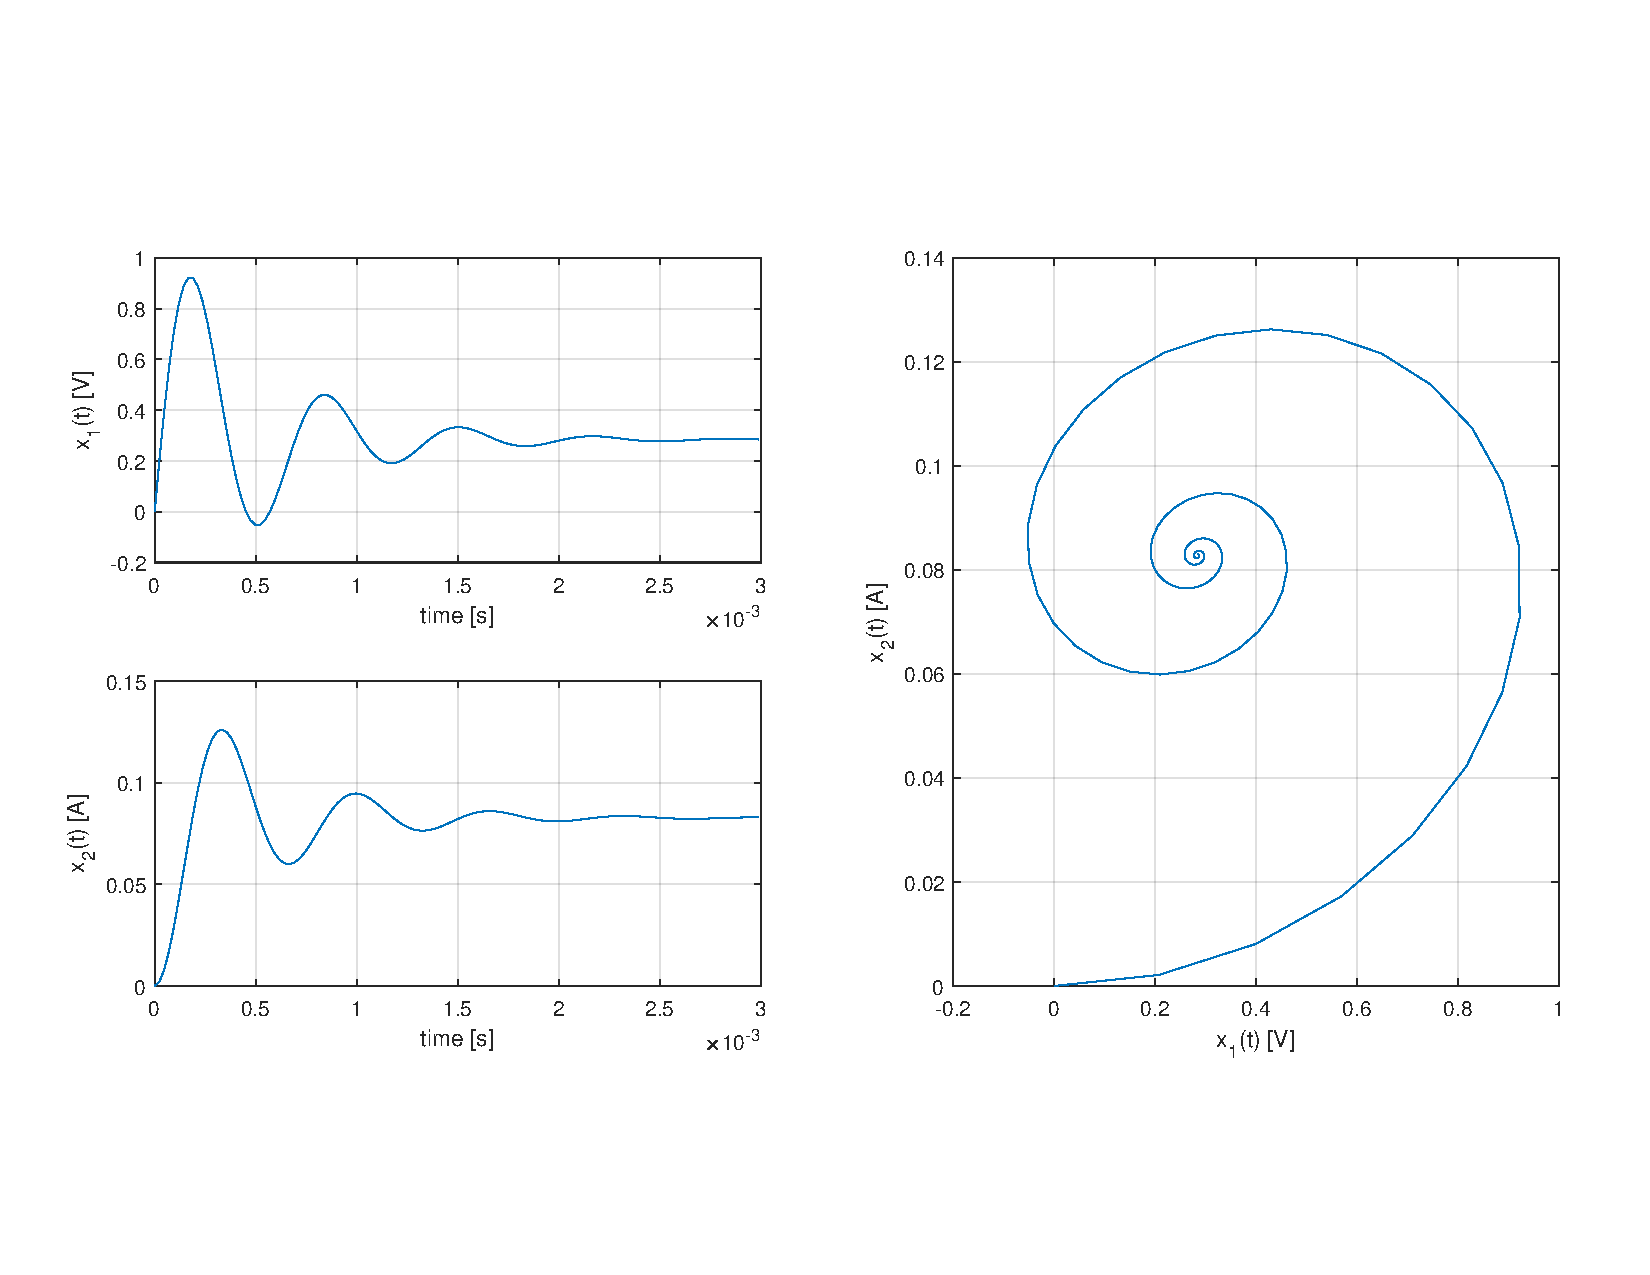
\includepdf[pages=-,pagecommand={},width=\textwidth]{matlab.pdf}
	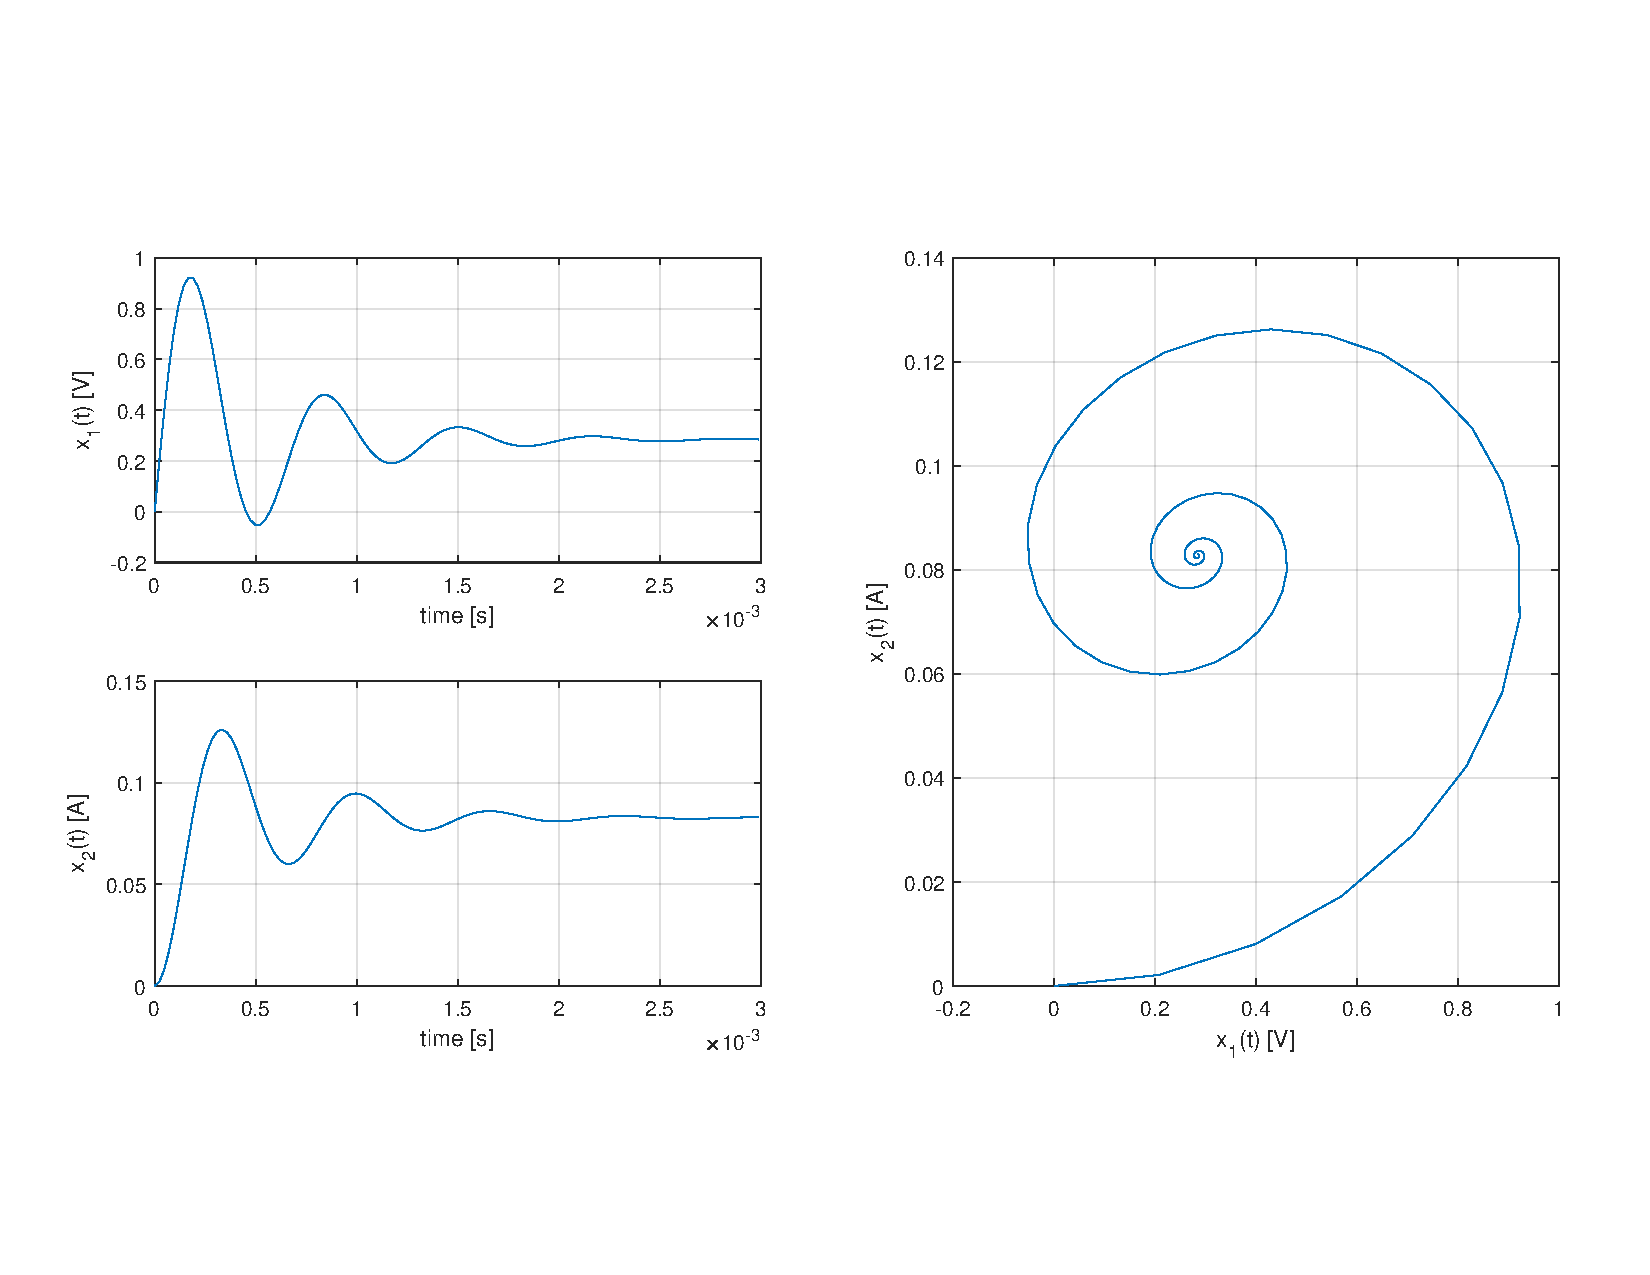
\includegraphics[width=\textwidth, trim=20 100 20 100, clip]{matlab.pdf}
	\caption{Output of the MATLAB simulation of the RLC step response.}
	\label{fig:matlab}
\end{figure}

\subsection{Conclusion}
%  conclusion of the exp
This experiment confirmed the state variable model, as well as the OrCAD model. The MATLAB simulation can be a valuable tool to solve for the step responses of linear circuits and can be more effective at determining behavior without using a full SPICE simulation.
\pagebreak

\section*{Appendix}
\begin{figure}[h]
	\centering
	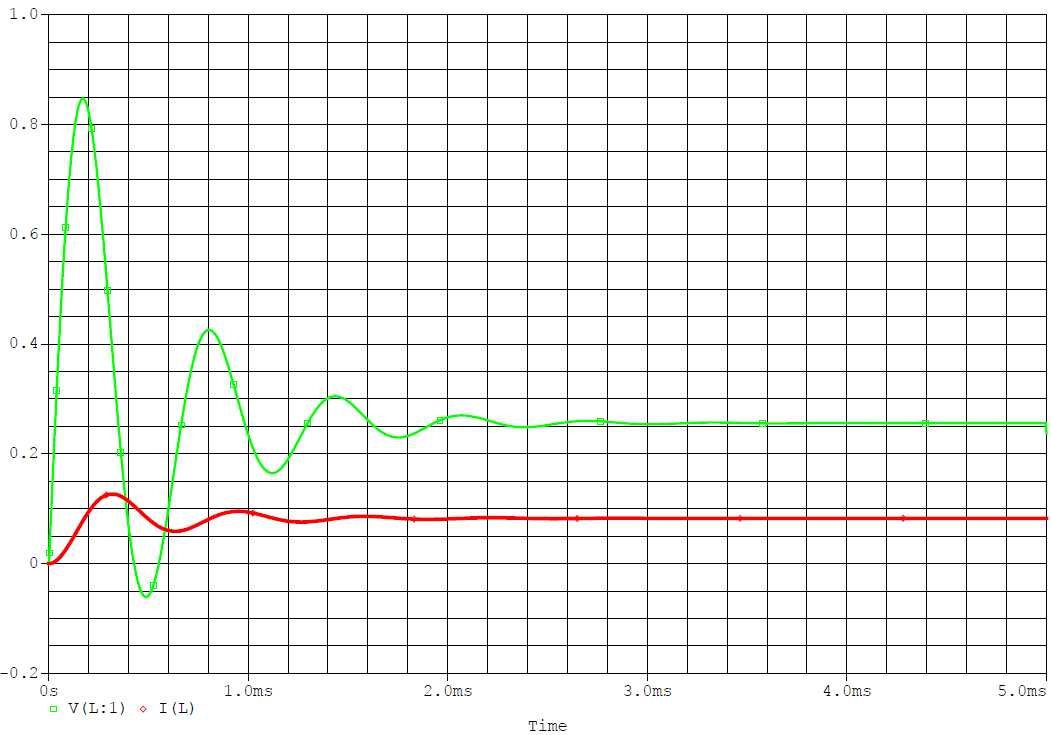
\includegraphics[width=1\linewidth]{rlcsim}
	\caption{Output of the OrCAD PSPICE step-response simulation.}
	\label{fig:rlcsim}
\end{figure}
\end{document}